% Created by tikzDevice version 0.12.6 on 2025-02-11 02:15:37
% !TEX encoding = UTF-8 Unicode
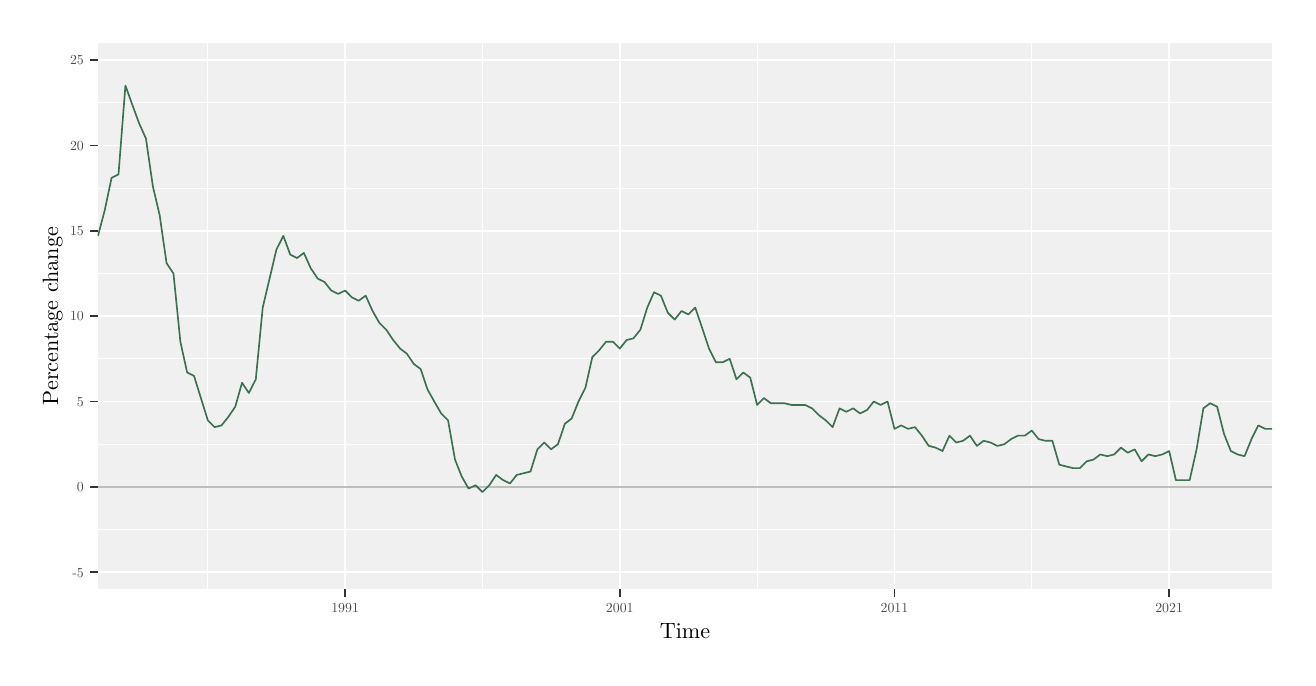
\begin{tikzpicture}[x=1pt,y=1pt]
\definecolor{fillColor}{RGB}{255,255,255}
\path[use as bounding box,fill=fillColor,fill opacity=0.00] (0,0) rectangle (455.30,227.65);
\begin{scope}
\path[clip] (  0.00,  0.00) rectangle (455.30,227.65);
\definecolor{drawColor}{RGB}{255,255,255}
\definecolor{fillColor}{RGB}{255,255,255}

\path[draw=drawColor,line width= 0.6pt,line join=round,line cap=round,fill=fillColor] (  0.00,  0.00) rectangle (455.30,227.65);
\end{scope}
\begin{scope}
\path[clip] ( 25.26, 24.68) rectangle (449.80,222.15);
\definecolor{fillColor}{gray}{0.94}

\path[fill=fillColor] ( 25.26, 24.68) rectangle (449.80,222.15);
\definecolor{drawColor}{RGB}{255,255,255}

\path[draw=drawColor,line width= 0.3pt,line join=round] ( 25.26, 46.28) --
	(449.80, 46.28);

\path[draw=drawColor,line width= 0.3pt,line join=round] ( 25.26, 77.13) --
	(449.80, 77.13);

\path[draw=drawColor,line width= 0.3pt,line join=round] ( 25.26,107.99) --
	(449.80,107.99);

\path[draw=drawColor,line width= 0.3pt,line join=round] ( 25.26,138.84) --
	(449.80,138.84);

\path[draw=drawColor,line width= 0.3pt,line join=round] ( 25.26,169.70) --
	(449.80,169.70);

\path[draw=drawColor,line width= 0.3pt,line join=round] ( 25.26,200.55) --
	(449.80,200.55);

\path[draw=drawColor,line width= 0.3pt,line join=round] ( 65.10, 24.68) --
	( 65.10,222.15);

\path[draw=drawColor,line width= 0.3pt,line join=round] (164.34, 24.68) --
	(164.34,222.15);

\path[draw=drawColor,line width= 0.3pt,line join=round] (263.59, 24.68) --
	(263.59,222.15);

\path[draw=drawColor,line width= 0.3pt,line join=round] (362.84, 24.68) --
	(362.84,222.15);

\path[draw=drawColor,line width= 0.6pt,line join=round] ( 25.26, 30.85) --
	(449.80, 30.85);

\path[draw=drawColor,line width= 0.6pt,line join=round] ( 25.26, 61.71) --
	(449.80, 61.71);

\path[draw=drawColor,line width= 0.6pt,line join=round] ( 25.26, 92.56) --
	(449.80, 92.56);

\path[draw=drawColor,line width= 0.6pt,line join=round] ( 25.26,123.42) --
	(449.80,123.42);

\path[draw=drawColor,line width= 0.6pt,line join=round] ( 25.26,154.27) --
	(449.80,154.27);

\path[draw=drawColor,line width= 0.6pt,line join=round] ( 25.26,185.12) --
	(449.80,185.12);

\path[draw=drawColor,line width= 0.6pt,line join=round] ( 25.26,215.98) --
	(449.80,215.98);

\path[draw=drawColor,line width= 0.6pt,line join=round] (114.71, 24.68) --
	(114.71,222.15);

\path[draw=drawColor,line width= 0.6pt,line join=round] (213.97, 24.68) --
	(213.97,222.15);

\path[draw=drawColor,line width= 0.6pt,line join=round] (313.21, 24.68) --
	(313.21,222.15);

\path[draw=drawColor,line width= 0.6pt,line join=round] (412.47, 24.68) --
	(412.47,222.15);
\definecolor{drawColor}{RGB}{190,190,190}

\path[draw=drawColor,line width= 0.6pt,line join=round] ( 25.26, 61.71) -- (449.80, 61.71);
\definecolor{drawColor}{RGB}{60,113,79}

\path[draw=drawColor,line width= 0.6pt,line join=round] ( 25.40,152.42) --
	( 27.85,161.68) --
	( 30.32,173.40) --
	( 32.82,174.63) --
	( 35.32,206.72) --
	( 37.76,199.94) --
	( 40.24,193.15) --
	( 42.74,187.59) --
	( 45.24,170.31) --
	( 47.71,159.82) --
	( 50.18,142.55) --
	( 52.68,138.84) --
	( 55.18,114.16) --
	( 57.63,103.05) --
	( 60.10,101.82) --
	( 62.60, 93.80) --
	( 65.10, 85.77) --
	( 67.54, 83.30) --
	( 70.02, 83.92) --
	( 72.52, 87.01) --
	( 75.02, 90.71) --
	( 77.46, 99.35) --
	( 79.93, 95.65) --
	( 82.43,100.58) --
	( 84.93,126.50) --
	( 87.41,136.99) --
	( 89.88,147.48) --
	( 92.38,152.42) --
	( 94.88,145.63) --
	( 97.32,144.40) --
	( 99.80,146.25) --
	(102.30,140.69) --
	(104.80,136.99) --
	(107.24,135.76) --
	(109.71,132.67) --
	(112.21,131.44) --
	(114.71,132.67) --
	(117.16,130.20) --
	(119.63,128.97) --
	(122.13,130.82) --
	(124.63,125.27) --
	(127.10,120.95) --
	(129.58,118.48) --
	(132.08,114.78) --
	(134.58,111.69) --
	(137.02,109.84) --
	(139.50,106.14) --
	(142.00,104.29) --
	(144.50, 96.88) --
	(146.94, 92.56) --
	(149.41, 88.24) --
	(151.91, 85.77) --
	(154.41, 71.58) --
	(156.86, 65.41) --
	(159.33, 61.09) --
	(161.83, 62.32) --
	(164.33, 59.85) --
	(166.80, 62.32) --
	(169.28, 66.03) --
	(171.78, 64.17) --
	(174.28, 62.94) --
	(176.72, 66.03) --
	(179.19, 66.64) --
	(181.69, 67.26) --
	(184.19, 75.28) --
	(186.64, 77.75) --
	(189.11, 75.28) --
	(191.61, 77.13) --
	(194.11, 84.54) --
	(196.56, 86.39) --
	(199.03, 92.56) --
	(201.53, 97.50) --
	(204.03,108.61) --
	(206.50,111.07) --
	(208.97,114.16) --
	(211.47,114.16) --
	(213.97,111.69) --
	(216.42,114.78) --
	(218.89,115.39) --
	(221.39,118.48) --
	(223.89,126.50) --
	(226.34,132.05) --
	(228.81,130.82) --
	(231.31,124.65) --
	(233.81,122.18) --
	(236.26,125.27) --
	(238.73,124.03) --
	(241.23,126.50) --
	(243.73,119.10) --
	(246.20,111.69) --
	(248.67,106.75) --
	(251.17,106.75) --
	(253.67,107.99) --
	(256.12,100.58) --
	(258.59,103.05) --
	(261.09,101.20) --
	(263.59, 91.33) --
	(266.04, 93.80) --
	(268.51, 91.94) --
	(271.01, 91.94) --
	(273.51, 91.94) --
	(275.95, 91.33) --
	(278.43, 91.33) --
	(280.93, 91.33) --
	(283.43, 90.09) --
	(285.90, 87.62) --
	(288.37, 85.77) --
	(290.87, 83.30) --
	(293.37, 90.09) --
	(295.82, 88.86) --
	(298.29, 90.09) --
	(300.79, 88.24) --
	(303.29, 89.48) --
	(305.73, 92.56) --
	(308.21, 91.33) --
	(310.71, 92.56) --
	(313.21, 82.69) --
	(315.65, 83.92) --
	(318.12, 82.69) --
	(320.62, 83.30) --
	(323.12, 80.22) --
	(325.60, 76.52) --
	(328.07, 75.90) --
	(330.57, 74.67) --
	(333.07, 80.22) --
	(335.52, 77.75) --
	(337.99, 78.37) --
	(340.49, 80.22) --
	(342.99, 76.52) --
	(345.43, 78.37) --
	(347.91, 77.75) --
	(350.41, 76.52) --
	(352.91, 77.13) --
	(355.35, 78.98) --
	(357.82, 80.22) --
	(360.32, 80.22) --
	(362.82, 82.07) --
	(365.30, 78.98) --
	(367.77, 78.37) --
	(370.27, 78.37) --
	(372.77, 69.73) --
	(375.21, 69.11) --
	(377.69, 68.49) --
	(380.19, 68.49) --
	(382.69, 70.96) --
	(385.13, 71.58) --
	(387.60, 73.43) --
	(390.10, 72.81) --
	(392.60, 73.43) --
	(395.05, 75.90) --
	(397.52, 74.05) --
	(400.02, 75.28) --
	(402.52, 70.96) --
	(404.99, 73.43) --
	(407.47, 72.81) --
	(409.97, 73.43) --
	(412.47, 74.67) --
	(414.91, 64.17) --
	(417.38, 64.17) --
	(419.88, 64.17) --
	(422.38, 75.28) --
	(424.83, 90.09) --
	(427.30, 91.94) --
	(429.80, 90.71) --
	(432.30, 80.84) --
	(434.75, 74.67) --
	(437.22, 73.43) --
	(439.72, 72.81) --
	(442.22, 78.98) --
	(444.69, 83.92) --
	(447.17, 82.69) --
	(449.67, 82.69);
\end{scope}
\begin{scope}
\path[clip] (  0.00,  0.00) rectangle (455.30,227.65);
\definecolor{drawColor}{gray}{0.30}

\node[text=drawColor,anchor=base east,inner sep=0pt, outer sep=0pt, scale=  0.50] at ( 20.31, 29.13) {-5};

\node[text=drawColor,anchor=base east,inner sep=0pt, outer sep=0pt, scale=  0.50] at ( 20.31, 59.98) {0};

\node[text=drawColor,anchor=base east,inner sep=0pt, outer sep=0pt, scale=  0.50] at ( 20.31, 90.84) {5};

\node[text=drawColor,anchor=base east,inner sep=0pt, outer sep=0pt, scale=  0.50] at ( 20.31,121.69) {10};

\node[text=drawColor,anchor=base east,inner sep=0pt, outer sep=0pt, scale=  0.50] at ( 20.31,152.55) {15};

\node[text=drawColor,anchor=base east,inner sep=0pt, outer sep=0pt, scale=  0.50] at ( 20.31,183.40) {20};

\node[text=drawColor,anchor=base east,inner sep=0pt, outer sep=0pt, scale=  0.50] at ( 20.31,214.26) {25};
\end{scope}
\begin{scope}
\path[clip] (  0.00,  0.00) rectangle (455.30,227.65);
\definecolor{drawColor}{gray}{0.20}

\path[draw=drawColor,line width= 0.6pt,line join=round] ( 22.51, 30.85) --
	( 25.26, 30.85);

\path[draw=drawColor,line width= 0.6pt,line join=round] ( 22.51, 61.71) --
	( 25.26, 61.71);

\path[draw=drawColor,line width= 0.6pt,line join=round] ( 22.51, 92.56) --
	( 25.26, 92.56);

\path[draw=drawColor,line width= 0.6pt,line join=round] ( 22.51,123.42) --
	( 25.26,123.42);

\path[draw=drawColor,line width= 0.6pt,line join=round] ( 22.51,154.27) --
	( 25.26,154.27);

\path[draw=drawColor,line width= 0.6pt,line join=round] ( 22.51,185.12) --
	( 25.26,185.12);

\path[draw=drawColor,line width= 0.6pt,line join=round] ( 22.51,215.98) --
	( 25.26,215.98);
\end{scope}
\begin{scope}
\path[clip] (  0.00,  0.00) rectangle (455.30,227.65);
\definecolor{drawColor}{gray}{0.20}

\path[draw=drawColor,line width= 0.6pt,line join=round] (114.71, 21.93) --
	(114.71, 24.68);

\path[draw=drawColor,line width= 0.6pt,line join=round] (213.97, 21.93) --
	(213.97, 24.68);

\path[draw=drawColor,line width= 0.6pt,line join=round] (313.21, 21.93) --
	(313.21, 24.68);

\path[draw=drawColor,line width= 0.6pt,line join=round] (412.47, 21.93) --
	(412.47, 24.68);
\end{scope}
\begin{scope}
\path[clip] (  0.00,  0.00) rectangle (455.30,227.65);
\definecolor{drawColor}{gray}{0.30}

\node[text=drawColor,anchor=base,inner sep=0pt, outer sep=0pt, scale=  0.50] at (114.71, 16.29) {1991};

\node[text=drawColor,anchor=base,inner sep=0pt, outer sep=0pt, scale=  0.50] at (213.97, 16.29) {2001};

\node[text=drawColor,anchor=base,inner sep=0pt, outer sep=0pt, scale=  0.50] at (313.21, 16.29) {2011};

\node[text=drawColor,anchor=base,inner sep=0pt, outer sep=0pt, scale=  0.50] at (412.47, 16.29) {2021};
\end{scope}
\begin{scope}
\path[clip] (  0.00,  0.00) rectangle (455.30,227.65);
\definecolor{drawColor}{RGB}{0,0,0}

\node[text=drawColor,anchor=base,inner sep=0pt, outer sep=0pt, scale=  0.80] at (237.53,  7.06) {Time};
\end{scope}
\begin{scope}
\path[clip] (  0.00,  0.00) rectangle (455.30,227.65);
\definecolor{drawColor}{RGB}{0,0,0}

\node[text=drawColor,rotate= 90.00,anchor=base,inner sep=0pt, outer sep=0pt, scale=  0.80] at ( 11.01,123.42) {Percentage change};
\end{scope}
\end{tikzpicture}
